\documentclass[]{article}

% Get better typography
\usepackage[protrusion=true,expansion=true]{microtype}		

% For algorithms
\usepackage[boxruled,linesnumbered,vlined,inoutnumbered]{algorithm2e}
\SetKwInOut{Parameter}{Parameters}

% For basic math, align, fonts, etc.
\usepackage{amsmath}
\usepackage{amssymb}
\usepackage{mathtools}
\usepackage{mathrsfs}
\usepackage{enumitem}

\DeclareMathOperator*{\argmin}{arg\,min}
\DeclareMathOperator*{\argmax}{arg\,max}

% For color
\usepackage{xcolor}
\usepackage{float}
\usepackage[top=2cm, bottom=2cm, left = 1cm, right = 1cm,columnsep=20pt]{geometry}
\definecolor{light-grey}{rgb}{0.9,0.9,0.9}
\definecolor{dark-red}{rgb}{0.4,0.15,0.15}
\definecolor{dark-blue}{rgb}{0,0,0.7}

% For links (e.g., clicking a reference takes you to the phy)
\usepackage{hyperref}
\hypersetup{
    colorlinks, linkcolor={dark-blue},
    citecolor={dark-blue}, urlcolor={dark-blue}
}

%-------------------------
%	BEGIN DOCUMENT / TITLE
%-------------------------
\begin{document}
\begin{center}
    \begin{Large}
    CMPSCI 687 Homework 4
    \end{Large}
    \\
    Due November 14, 2019, 11:55pm Eastern Time
\end{center}
\addcontentsline{toc}{subsection}{\textbf{Homework 4}}

\noindent {\bf Instructions: } Collaboration is not allowed on any part of this assignment. Submissions must be typed (hand written and scanned submissions will not be accepted). You must use \LaTeX. The assignment should be submitted as five documents: a .pdf with your written answers, two .hpp files, and two .cpp files as described in the programming portion.
\\\\
\section*{Programming (75 Points Total)}

In this assignment, you will implement Sarsa and $Q$-learning, and will apply them to a gridworld (not the one from the course notes), mountain car, acrobot, and cart-pole. Begin with the source code provided \href{https://people.cs.umass.edu/~pthomas/courses/CMPSCI_687_Fall2019/HW4Source.zip}{here} (see the previous assignments for instructions regarding opening the project). Look at main.cpp, starting with the function main. Look through how this code functions: it applies Sarsa and Q-learning to various MDPs in sequence. Hyperparameters (not good ones!) are specified for each environment in main.cpp.\footnote{For this assignment, you may view the iOrder and dOrder hyperparameters as both being the order of the Fourier basis, and you may always set them to the same value.} The code for Sarsa should be in Sarsa.hpp (a header file, that defines the Sarsa class) and Sarsa.cpp (the source file, that includes the actual code for all of the functions that a Sarsa object requires). Similarly the code for Q-learning is split across QLearning.hpp and QLearning.cpp. You should fill code into Sarsa.hpp, Sarsa.cpp, QLearning.hpp, and QLearning.cpp, and these four files are the four that you should submit with your assignment.

To be clear, your edits should be: 1) changing the hyperparameters specified in main.cpp (you do not have to submit these, but will report hyper-parameter values in your write-up), 2) adding code to the train function in QLearning.cpp (you may change QLearning.hpp and other functions in QLearning.cpp, but this is not necessary), 3) adding code to Sarsa.hpp (private member variables) and Sarsa.cpp (likely all of the functions except for ``getAction'' will have code that you add).

After reading through main.cpp to see what it does, look through Gridworld.hpp and Gridworld.cpp. Gridworld.hpp and Gridworld.cpp have been commented more heavily than the files for the other MDPs. These provide an example of a class in C++. The .hpp file contains the definition of the Gridworld object, and the .cpp file implements the functions that it requires. This also shows how the environments all work. Notice, for example, that the getState() function normalizes the state for you -- it returns the state as a vector, each element of which is in the interval $[0,1]$. Notice also that this code is set up to work well with linear function approximation, as the state is a vector of floating point numbers (not yet features!) that can be provided to the FourierBasis class to convert to features.

Now that you've read through main.cpp and Gridworld.cpp, look at QLearning.hpp and QLearning.cpp. QLearning.hpp and QLearning.cpp have been commented more heavily than the files for Sarsa. Most of this class is implemented for you. The ``train'' function has not been implemented fully -- you must fill this in. Notice some useful functions have been provided in MathUtils.hpp, like ``dot''. Also, note that this time we are not using the Eigen library. Don't be afraid to use for loops though, as these are very efficient in C++. The computational bottleneck in this code is usually computing the cosines in the FourierBasis object. This is why we compute and store the features for state $s'$ in an $(s,a,r,s')$ tuple, so that we can re-use them at the next iteration for state $s$. We could be even more efficient by not recomputing features whenever the agent is asked for an action (right now, QLearning will compute features for state $s$ twice, once in the train function and once in the getAction function). For this assignment, this inefficiency is ok.

Once you have implemented the train function in QLearning.cpp, try setting the hyperparemeters in main.cpp to get results similar to those in the provided file ``plots.xlsx''. If, after running your code, you copy the contents of the other .csv files over the entries in plots.xlsx, it should update to show the plots we want. You are welcome to use your own system (e.g., write your own python code) to make plots from the output .xlsx files. Hint: For both Q-Learning and Sarsa, set $q(s',a')=0$ when computing the TD-error if $s'$ is a terminal state, since we know this action-value and therefore do not need to approximate it.

Next, look at Sarsa.hpp and Sarsa.cpp. These are left more empty for you to fill in. Importantly, we're making this harder for you that just putting in the pseudocode. Look back at Section 3.1. The pseudocode there works well for Q-learning, but not as well for Sarsa, since Sarsa requires the action $a'$ to update. Notice that main.cpp implements the pseudocode from Section 3.1. So, you must write Sarsa in a way that works with this setup. Hint: you will want the agent to have some memory, perhaps remembering which states, actions, and/or rewards it saw previously.

Point allocations for this assignment will be determined at the time of grading, based on which mistakes and issues are common.

\begin{enumerate}
    \item Describe the process of implementing Q-Learning. Did everything work immediately? Did you have bugs that you had to fix? What were they?

	{
		\color{blue}
		Ans 1. I implemented Q-Learning looking at the pseudocode provided in the notes. I did not modify QLearning.hpp but I have modified QLearning.cpp to complete the QLearning algorithm. Firstly, we compute TD-error outside the for loop. We use the TD-error formula for the TD-error which is the current reward + $\gamma$ * max over actions (q(next state, action at next time step)) - q(current state, current action). Although, for the terminal state, the TD-error becomes only current reward - q(current state, current action). Then, in the for loop, we do the TD-update step for all features as w[current action][feature] += $\alpha$ * TD-error * phi[feature].

The program was really simple to implement, so I only had one error. The error was that instead of having w[current action][feature] += $\alpha$ * TD-error * phi[feature], I mistakenly implemented w[current action][feature] = $\alpha$ * TD-error * phi[feature] at first. I quickly noticed that and rectified it. This was the only error I had while implementing the Q-Learning algorithm. After I fixed this bug, everything worked immediately.

	}

    \item Describe the process of implementing Sarsa. Did everything work immediately? Did you have bugs that you had to fix? What were they?

	{
		\color{blue}
		Ans 2. I implemented Sarsa looking at the pseudocode provided in the notes and looking at the formulas and modifying the implementation in the notes a bit, as the given code does not exactly emulate the pseudocode provided in the notes. I modified Sarsa.hpp by adding a four private variables to store vector$<double>$ phi\_s, bool initialization flag, int previous action, and double previous reward. I have also modified Sarsa.cpp to complete the Sarsa algorithm. In the newEpisode function, I have set the initialization flag to false to mark the start of a new episode. In the train function, I have just stored the initial action, initial state, initial phi, and set the initialization flag to true to indicate that we can perform the TD computation for the future time steps. So, when the train function is called for the first time step of a new episode, we do not do any TD computation other than just storing the variables to use them from the next time step. For all time steps other than the initialization time step, in which the bool initialization flag is set to true, compute the TD-error outside the for loop. We use the TD-error formula for the TD-error which is the previous reward + $\gamma$ * q(current state, current action) - q(previous state, previous action). Then, in the for loop, we do the TD-update step for the previous time step for all features as w[previous action][feature] += $\alpha$ * TD-error * phi[feature]. Although, when $s'$ is terminal, we also need to do the TD-error computation and the TD-update for the last step. The TD-error outside the for loop when $s'$ is terminal is the current reward - q(current state, current action). Then, in the for loop, we do the TD-update step for all features as w[current action][feature] += $\alpha$ * TD-error * phi[feature].

I had a bug in my implementation in which I did not set the initialization flag to false in the newEpisode function. I quickly noticed that and rectified it. This was the only error I had while implementing the Q-Learning algorithm. After I fixed this bug, everything worked immediately.

	}

    \item Describe the process of optimizing the hyperparameters for Q-Learning for MountainCar, and report the final hyperparameters that you found.

	{
		\color{blue}
		Ans 3. After implementing Q-Learning, I ran the Q-Learning algorithm for the MountainCar environment. In order to tune the hyperparameters to give good convergence result (high expected return), I did a grid search on the hyperparameters by having numerous combinations of floating point numbers of these hyperparameters. I used the number of trials ($numTrials$) = 100, the number of episodes ($numEpisodes$) = 40, and the maximum length of each episode ($maxEpisodeLength$) = 20000 throughout the process of tuning hyperparameters for Q-Learning for the MountainCar environment. The five other hyperparameters, $\alpha$, $\gamma$, $\epsilon$, $iOrder$, and $dOrder$ took values from sets of numerous floating point numbers. Precisely, I tried each combination of $\alpha$, $\gamma$, $\epsilon$, $iOrder$, and $dOrder$ (through nested for loops) for $\alpha \in \{0.01, 0.02, 0.03\}$, $\gamma \in \{1.0\}$, $\epsilon \in \{0.1, 0.2, 0.3\}$, $iOrder \in \{1, 2\}$, and $dOrder \in \{1\}$. Among 18 of these combinations, the best combination of hyperparameters I found have $\alpha$ = 0.02, $\gamma$ = 1.0, $\epsilon$ = 0.1, $iOrder$ = 1, $dOrder$ =  1, $numTrials$ = 100, $numEpisodes$ = 40, and $maxEpisodeLength$ = 20000. The algorithm converged to an expected return of -141.420000, which is better than the expected return of -171.3 of the sample plot.

	}

    \item Describe the process of optimizing the hyperparameters for Q-Learning for CartPole, and report the final hyperparameters that you found.

	{
		\color{blue}
		Ans 4. After implementing Q-Learning, I ran the Q-Learning algorithm for the CartPole environment. In order to tune the hyperparameters to give good convergence result (high expected return), I did a grid search on the hyperparameters by having numerous combinations of floating point numbers of these hyperparameters. I used the number of trials ($numTrials$) = 50, the number of episodes ($numEpisodes$) = 50, and the maximum length of each episode ($maxEpisodeLength$) = INT\_MAX throughout the process of tuning hyperparameters for Q-Learning for the CartPole environment. The five other hyperparameters, $\alpha$, $\gamma$, $\epsilon$, $iOrder$, and $dOrder$ took values from sets of numerous floating point numbers. Precisely, I tried each combination of $\alpha$, $\gamma$, $\epsilon$, $iOrder$, and $dOrder$ (through nested for loops) for $\alpha \in \{0.002, 0.004, 0.006\}$, $\gamma \in \{1.0\}$, $\epsilon \in \{0.1, 0.2\}$, $iOrder \in \{2, 4, 6\}$, and $dOrder \in \{1, 2\}$. Among 36 of these combinations, the best combination of hyperparameters I found have $\alpha$ = 0.006, $\gamma$ = 1.0, $\epsilon$ = 0.1, $iOrder$ = 4, $dOrder$ =  2, $numTrials$ = 50, $numEpisodes$ = 50, and $maxEpisodeLength$ = INT\_MAX. The algorithm converged to an expected return of 943.440000, which is near the expected return of 957.4 of the sample plot.

	}

    \item Describe the process of optimizing the hyperparameters for Q-Learning for Acrobot, and report the final hyperparameters that you found.

	{
		\color{blue}
		Ans 5. After implementing Q-Learning, I ran the Q-Learning algorithm for the Acrobot environment. In order to tune the hyperparameters to give good convergence result (high expected return), I did a grid search on the hyperparameters by having numerous combinations of floating point numbers of these hyperparameters. I used the number of trials ($numTrials$) = 100, the number of episodes ($numEpisodes$) = 100, and the maximum length of each episode ($maxEpisodeLength$) = 3000 throughout the process of tuning hyperparameters for Q-Learning for the Acrobot environment. The five other hyperparameters, $\alpha$, $\gamma$, $\epsilon$, $iOrder$, and $dOrder$ took values from sets of numerous floating point numbers. Precisely, I tried each combination of $\alpha$, $\gamma$, $\epsilon$, $iOrder$, and $dOrder$ (through nested for loops) for $\alpha \in \{0.01, 0.001, 0.0001\}$, $\gamma \in \{1.0\}$, $\epsilon \in \{0.3, 0.4\}$, $iOrder \in \{3, 4, 5\}$, and $dOrder \in \{0\}$. Among 18 of these combinations, the best combination of hyperparameters I found have $\alpha$ = 0.001, $\gamma$ = 1.0, $\epsilon$ = 0.3, $iOrder$ = 4, $dOrder$ =  0, $numTrials$ = 100, $numEpisodes$ = 100, and $maxEpisodeLength$ = 3000. The algorithm converged to an expected return of -6.732000, which is better than the expected return of -13.045 of the sample plot.

	}

    \item Describe the process of optimizing the hyperparameters for Q-Learning for Gridworld, and report the final hyperparameters that you found.

	{
		\color{blue}
		Ans 6. After implementing Q-Learning, I ran the Q-Learning algorithm for the Gridworld environment. In order to tune the hyperparameters to give good convergence result (high expected return), I did a grid search on the hyperparameters by having numerous combinations of floating point numbers of these hyperparameters. I used the number of trials ($numTrials$) = 100, the number of episodes ($numEpisodes$) = 20, and the maximum length of each episode ($maxEpisodeLength$) = 1000 throughout the process of tuning hyperparameters for Q-Learning for the Gridworld environment. The five other hyperparameters, $\alpha$, $\gamma$, $\epsilon$, $iOrder$, and $dOrder$ took values from sets of numerous floating point numbers. Precisely, I tried each combination of $\alpha$, $\gamma$, $\epsilon$, $iOrder$, and $dOrder$ (through nested for loops) for $\alpha \in \{0.01, 0.02, 0.03\}$, $\gamma \in \{1.0\}$, $\epsilon \in \{0.1, 0.2\}$, $iOrder \in \{1, 2, 3\}$, and $dOrder \in \{0\}$. Among 18 of these combinations, the best combination of hyperparameters I found have $\alpha$ = 0.01, $\gamma$ = 1.0, $\epsilon$ = 0.1, $iOrder$ = 3, $dOrder$ =  0, $numTrials$ = 100, $numEpisodes$ = 20, and $maxEpisodeLength$ = 1000. The algorithm converged to an expected return of -11.430000, which is better than the expected return of -11.47 of the sample plot.

	}

    \item Describe the process of optimizing the hyperparameters for Sarsa for MountainCar, and report the final hyperparameters that you found.

	{
		\color{blue}
		Ans 7. After implementing Sarsa, I ran the Sarsa algorithm for the MountainCar environment. In order to tune the hyperparameters to give good convergence result (high expected return), I did a grid search on the hyperparameters by having numerous combinations of floating point numbers of these hyperparameters. I used the number of trials ($numTrials$) = 100, the number of episodes ($numEpisodes$) = 40, and the maximum length of each episode ($maxEpisodeLength$) = 20000 throughout the process of tuning hyperparameters for Q-Learning for the MountainCar environment. The five other hyperparameters, $\alpha$, $\gamma$, $\epsilon$, $iOrder$, and $dOrder$ took values from sets of numerous floating point numbers. Precisely, I tried each combination of $\alpha$, $\gamma$, $\epsilon$, $iOrder$, and $dOrder$ (through nested for loops) for $\alpha \in \{0.01, 0.02, 0.03\}$, $\gamma \in \{1.0\}$, $\epsilon \in \{0.1, 0.2, 0.3\}$, $iOrder \in \{1, 2\}$, and $dOrder \in \{1\}$. Among 18 of these combinations, the best combination of hyperparameters I found have $\alpha$ = 0.02, $\gamma$ = 1.0, $\epsilon$ = 0.1, $iOrder$ = 1, $dOrder$ =  1, $numTrials$ = 100, $numEpisodes$ = 40, and $maxEpisodeLength$ = 20000. The algorithm converged to an expected return of -145.130000, which is better than the expected return of -173.54 of the sample plot.
	}

    \item Describe the process of optimizing the hyperparameters for Sarsa for CartPole, and report the final hyperparameters that you found.

	{
		\color{blue}
		Ans 8. After implementing Sarsa, I ran the Sarsa algorithm for the CartPole environment. In order to tune the hyperparameters to give good convergence result (high expected return), I did a grid search on the hyperparameters by having numerous combinations of floating point numbers of these hyperparameters. I used the number of trials ($numTrials$) = 50, the number of episodes ($numEpisodes$) = 50, and the maximum length of each episode ($maxEpisodeLength$) = INT\_MAX throughout the process of tuning hyperparameters for Sarsa for the CartPole environment. The five other hyperparameters, $\alpha$, $\gamma$, $\epsilon$, $iOrder$, and $dOrder$ took values from sets of numerous floating point numbers. Precisely, I tried each combination of $\alpha$, $\gamma$, $\epsilon$, $iOrder$, and $dOrder$ (through nested for loops) for $\alpha \in \{0.004, 0.006, 0.008\}$, $\gamma \in \{1.0\}$, $\epsilon \in \{0.1, 0.2\}$, $iOrder \in \{1, 2\}$, and $dOrder \in \{1, 2\}$. Among 24 of these combinations, the best combination of hyperparameters I found have $\alpha$ = 0.008, $\gamma$ = 1.0, $\epsilon$ = 0.1, $iOrder$ = 2, $dOrder$ =  2, $numTrials$ = 50, $numEpisodes$ = 50, and $maxEpisodeLength$ = INT\_MAX. The algorithm converged to an expected return of 904.580000, which is better than the expected return of 861.4 of the sample plot.

	}

    \item Describe the process of optimizing the hyperparameters for Sarsa for Acrobot, and report the final hyperparameters that you found.

	{
		\color{blue}
		Ans 9. After implementing Sarsa, I ran the Sarsa algorithm for the Acrobot environment. In order to tune the hyperparameters to give good convergence result (high expected return), I did a grid search on the hyperparameters by having numerous combinations of floating point numbers of these hyperparameters. I used the number of trials ($numTrials$) = 100, the number of episodes ($numEpisodes$) = 100, and the maximum length of each episode ($maxEpisodeLength$) = 3000 throughout the process of tuning hyperparameters for Sarsa for the Acrobot environment. The five other hyperparameters, $\alpha$, $\gamma$, $\epsilon$, $iOrder$, and $dOrder$ took values from sets of numerous floating point numbers. Precisely, I tried each combination of $\alpha$, $\gamma$, $\epsilon$, $iOrder$, and $dOrder$ (through nested for loops) for $\alpha \in \{0.01, 0.02, 0.03\}$, $\gamma \in \{1.0\}$, $\epsilon \in \{0.04, 0.05, 0.06\}$, $iOrder \in \{3, 4\}$, and $dOrder \in \{0\}$. Among 18 of these combinations, the best combination of hyperparameters I found have $\alpha$ = 0.001, $\gamma$ = 1.0, $\epsilon$ = 0.04, $iOrder$ = 4, $dOrder$ =  0, $numTrials$ = 100, $numEpisodes$ = 100, and $maxEpisodeLength$ = 3000. The algorithm converged to an expected return of -3.853000, which is better than the expected return of -9.335 of the sample plot.
	}

    \item Describe the process of optimizing the hyperparameters for Sarsa for Gridworld, and report the final hyperparameters that you found.

	{
		\color{blue}
		Ans 10. After implementing Sarsa, I ran the Sarsa algorithm for the Gridworld environment. In order to tune the hyperparameters to give good convergence result (high expected return), I did a grid search on the hyperparameters by having numerous combinations of floating point numbers of these hyperparameters. I used the number of trials ($numTrials$) = 100, the number of episodes ($numEpisodes$) = 20, and the maximum length of each episode ($maxEpisodeLength$) = 1000 throughout the process of tuning hyperparameters for Sarsa for the Gridworld environment. The five other hyperparameters, $\alpha$, $\gamma$, $\epsilon$, $iOrder$, and $dOrder$ took values from sets of numerous floating point numbers. Precisely, I tried each combination of $\alpha$, $\gamma$, $\epsilon$, $iOrder$, and $dOrder$ (through nested for loops) for $\alpha \in \{0.01, 0.02, 0.03\}$, $\gamma \in \{1.0\}$, $\epsilon \in \{0.01, 0.02, 0.03\}$, $iOrder \in \{1, 2\}$, and $dOrder \in \{0\}$. Among 18 of these combinations, the best combination of hyperparameters I found have $\alpha$ = 0.02, $\gamma$ = 1.0, $\epsilon$ = 0.01, $iOrder$ = 1, $dOrder$ =  0, $numTrials$ = 100, $numEpisodes$ = 20, and $maxEpisodeLength$ = 1000. The algorithm converged to an expected return of -8.270000, which is better than the expected return of -39.63 of the sample plot.

	}

    \item Provide four plots, one per environment, showing the learning curves for Sarsa and Q-learning with the best hyperparameters that you found. Keep the number of trials, number of episodes, and maxEpisodeLength terms from the provided main.cpp. Include error bars showing one standard deviation. These plots can be created using any plotting software of your choice.

	{
		\color{blue}
		Ans 11. The best combination of hyperparameters I found for the Mountain Car environment with Q-Learning have $\alpha$ = 0.02, $\gamma$ = 1.0, $\epsilon$ = 0.1, $iOrder$ = 1, $dOrder$ =  1, $numTrials$ = 100, $numEpisodes$ = 40, and $maxEpisodeLength$ = 20000.
The best combination of hyperparameters I found for the Mountain Car environment with Sarsa have $\alpha$ = 0.02, $\gamma$ = 1.0, $\epsilon$ = 0.1, $iOrder$ = 1, $dOrder$ =  1, $numTrials$ = 100, $numEpisodes$ = 40, and $maxEpisodeLength$ = 20000.
These best hyperparameters are used to plot the learning curves for the Mountain Car environment using Q-Learning and Sarsa.
		
		\begin{figure}[H]
		    \centering
		    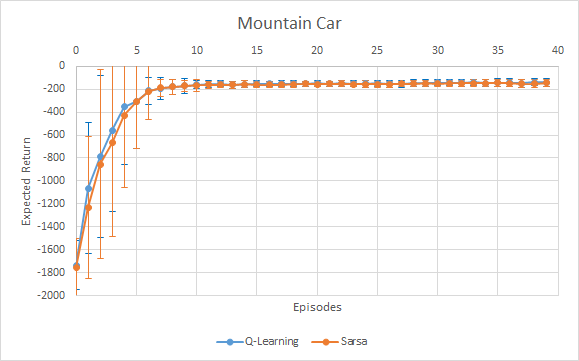
\includegraphics[width=0.5\textwidth]{MountainCar.png}
		    \caption{Learning curves for the Mountain Car environment plot with Q-Learning and Sarsa using the best hyperparameters found. The Q-Learning algorithm is plotted using blue color and the Sarsa algorithm is plotted using orange color. Error bars included showing one standard deviation. The plot has converged to an expected return of -141.42 for Q-Learning and to an expected return of -145.13 for Sarsa.}
		    \label{fig: Mountain Car environment plot with Q-Learning and Sarsa}
		\end{figure}

The best combination of hyperparameters I found for the CartPole environment with Q-Learning have $\alpha$ = 0.006, $\gamma$ = 1.0, $\epsilon$ = 0.1, $iOrder$ = 4, $dOrder$ =  2, $numTrials$ = 50, $numEpisodes$ = 50, and $maxEpisodeLength$ = INT\_MAX.
The best combination of hyperparameters I found for the CartPole environment with Sarsa have $\alpha$ = 0.008, $\gamma$ = 1.0, $\epsilon$ = 0.1, $iOrder$ = 2, $dOrder$ =  2, $numTrials$ = 50, $numEpisodes$ = 50, and $maxEpisodeLength$ = INT\_MAX.
These best hyperparameters are used to plot the learning curves for the CartPole environment using Q-Learning and Sarsa.
		
		\begin{figure}[H]
		    \centering
		    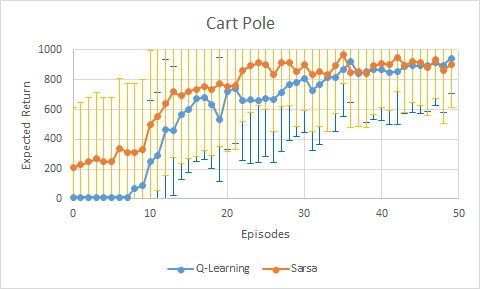
\includegraphics[width=0.5\textwidth]{Cartpole.png}
		    \caption{Learning curves for the CartPole environment plot with Q-Learning and Sarsa using the best hyperparameters found. The Q-Learning algorithm is plotted using blue color and the Sarsa algorithm is plotted using orange color. Error bars included showing one standard deviation. The plot has converged to an expected return of 943.44 for Q-Learning and to an expected return of 904.58 for Sarsa.}
		    \label{fig: Cross Entropy Method algorithm for More-Watery 687-Gridworld}
		\end{figure}

The best combination of hyperparameters I found for the Acrobot environment with Q-Learning have $\alpha$ = 0.001, $\gamma$ = 1.0, $\epsilon$ = 0.3, $iOrder$ = 4, $dOrder$ =  0, $numTrials$ = 100, $numEpisodes$ = 100, and $maxEpisodeLength$ = 3000.
The best combination of hyperparameters I found for the Acrobot environment with Sarsa have $\alpha$ = 0.001, $\gamma$ = 1.0, $\epsilon$ = 0.04, $iOrder$ = 4, $dOrder$ =  0, $numTrials$ = 100, $numEpisodes$ = 100, and $maxEpisodeLength$ = 3000.
These best hyperparameters are used to plot the learning curves for the Acrobot environment using Q-Learning and Sarsa.
		
		\begin{figure}[H]
		    \centering
		    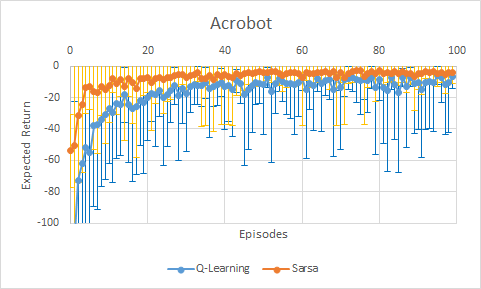
\includegraphics[width=0.5\textwidth]{Acrobot.png}
		    \caption{Learning curves for the Acrobot environment plot with Q-Learning and Sarsa using the best hyperparameters found. The Q-Learning algorithm is plotted using blue color and the Sarsa algorithm is plotted using orange color. Error bars included showing one standard deviation. The plot has converged to an expected return of -6.732 for Q-Learning and to an expected return of -3.853 for Sarsa.}
		    \label{fig: Acrobot environment plot with Q-Learning and Sarsa}
		\end{figure}

The best combination of hyperparameters I found for the Gridworld environment with Q-Learning have $\alpha$ = 0.01, $\gamma$ = 1.0, $\epsilon$ = 0.1, $iOrder$ = 3, $dOrder$ =  0, $numTrials$ = 100, $numEpisodes$ = 20, and $maxEpisodeLength$ = 1000.
The best combination of hyperparameters I found for the Gridworld environment with Sarsa have $\alpha$ = 0.02, $\gamma$ = 1.0, $\epsilon$ = 0.01, $iOrder$ = 1, $dOrder$ =  0, $numTrials$ = 100, $numEpisodes$ = 20, and $maxEpisodeLength$ = 1000.
These best hyperparameters are used to plot the learning curves for the Gridworld environment using Q-Learning and Sarsa.
		
		\begin{figure}[H]
		    \centering
		    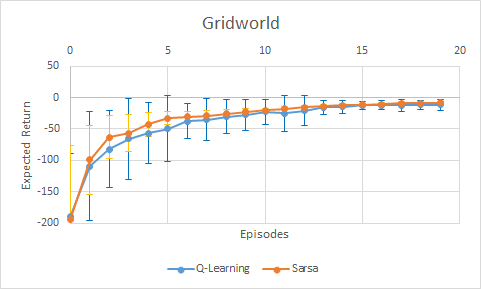
\includegraphics[width=0.5\textwidth]{Gridworld.png}
		    \caption{Learning curves for the Gridworld environment plot with Q-Learning and Sarsa using the best hyperparameters found. The Q-Learning algorithm is plotted using blue color and the Sarsa algorithm is plotted using orange color. Error bars included showing one standard deviation. The plot has converged to an expected return of -11.43 for Q-Learning and to an expected return of -8.27 for Sarsa.}
		\end{figure}

	}

    \item Compare your experiences with Q-Learning and Sarsa to your experiences with BBO. Which did you find easier to get working? Which algorithms learned fastest on Cart-Pole (in HW2, you implemented BBO algorithms for Cart-Pole)?

	{
		\color{blue}
		Ans 12. I have compared the experiences with Q-Learning and Sarsa to the experiences with BBO. It was significantly easier and faster to get Q-Learning and Sarsa working than any of the BBO algorithms (First-Choice Hill Climbing, Cross-Entropy Method, or Genetic Algorithm). This is because Q-Learning and Sarsa were easier to implement and finished running significantly faster and took much fewer number of episodes to converge to optimal values of expected returns for few a combinations of hyperparameters (best hyperparameters) than any of the BBO algorithm, that it was faster to try different combinations of hyperparameters and find the best sets of hyperparameters. In sum, Q-Learning and Sarsa learned much faster on Cart-Pole than any of the BBO algorithms implemented for Cart-Pole in HW2.

	}

    \item Be sure to submit your QLearning.hpp (even if it is unchanged, as recommended), QLearning.cpp, Sarsa.hpp, and Sarsa.cpp files with your write-up.

	{
		\color{blue}
		Ans 13. I have made sure to submit the QLearning.hpp (even if it is unchanged, as recommended), QLearning.cpp, Sarsa.hpp, and Sarsa.cpp files with the write-up.

	}

\end{enumerate}

Note: This code is written to be relatively simple, as many of you are new to C++. This does not represent best coding practices (e.g., we could make use of subclasses).

\end{document}
